\subsection{Motorenansteuerung}\label{subsec:Hardware_Motorenansteuerung}

Im Folgenden wird die Motorenansteuerung verifiziert. Die Ansteuerung gliedert sich in zwei Teile, einerseits das Feedback, andererseits der Motorentreiber. Deshalb wird nur auf diese Bereiche eingegangen.

\subsubsection{Resolver}\label{subsubsec:Hardware_Resolver}

Der Ausgang des PWM-Pins beträgt 8kHz, wie in den Abbildungen \ref{fig:Hardware_Resolver_Interface_0_0} und \ref{fig:Hardware_Resolver_Interface_0_1} ersichtlich.


\begin{figure}[h!]
\centering
\subcaptionbox{Ausgangssignal des PWM-Pins beim Einschaltvorgang.\label{fig:Hardware_Resolver_Interface_0_0}}{	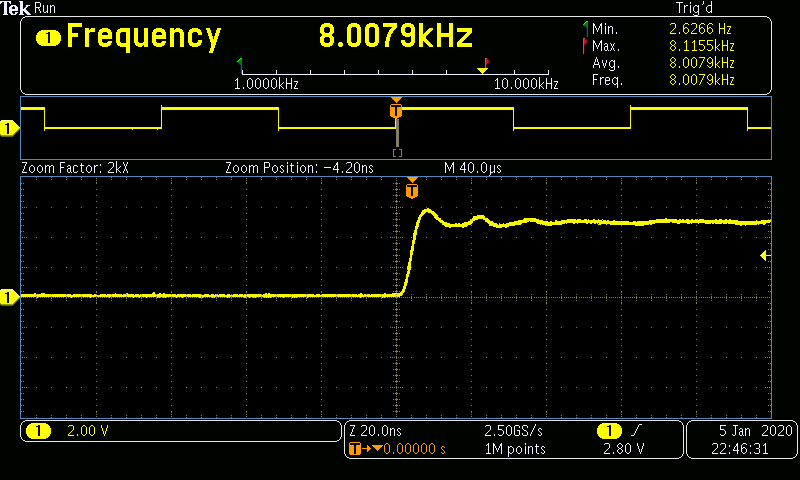
\includegraphics[width=0.45\textwidth]{graphics/Messung_Resolver_Interface_0_0.png}}
\hfill
\subcaptionbox{Ausgangssignal des PWM-Pins beim Ausschaltvorgang.\label{fig:Hardware_Resolver_Interface_0_1}}{	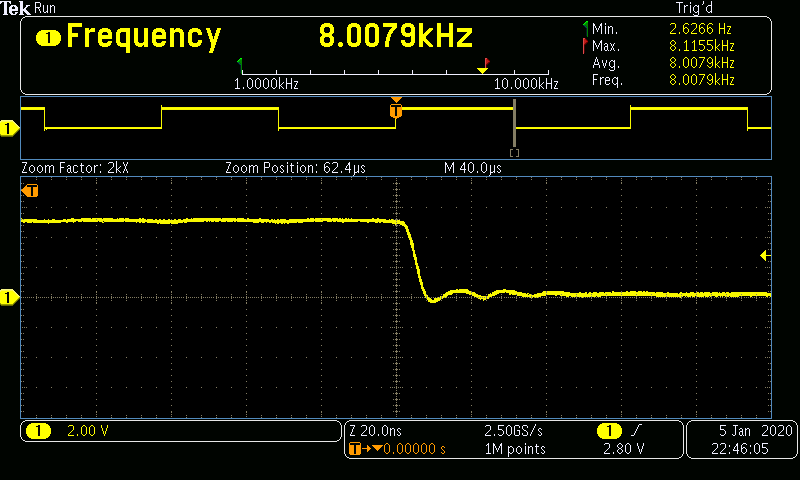
\includegraphics[width=0.45\textwidth]{graphics/Messung_Resolver_Interface_0_1.png}}
\hfill
\caption{Schematische und grafische Darstellung eines Resolvers.}
\label{fig:Hardware_Resolver_Interface_0}
\end{figure}

Das nachgebaute Resolver-Interface ergab folgende Messungen:

Abbildung \ref{fig:Hardware_Resolver_Interface_1} zeigt das PWM-Signal hinter dem Kondensator. Das hier anliegende Signal wird über dem Opamp integriert.

\begin{figure}[h!]
	\centering
	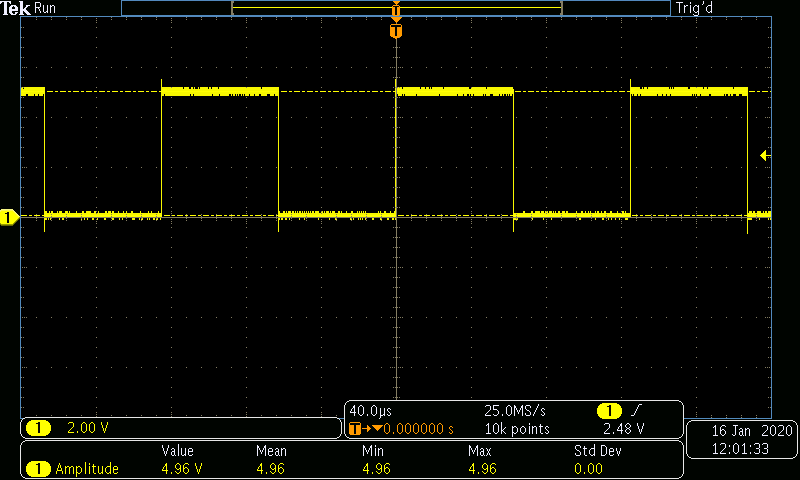
\includegraphics[width=0.8\textwidth]{graphics/Resolver_Rechteck.png}
	\caption{Messung zwischen Opamp U1 und Widerstand R4.} 
	\label{fig:Hardware_Resolver_Interface_1}
\end{figure}

Das Integrierte Signal ist in Abbildung \ref{fig:Hardware_Resolver_Interface_2} zu erkennen. Die Amplitude beträgt 3.12V, dies liegt am Maximalwert der Spannungsspitze, ansonsten entspricht die Messung der Erwartung aufgrund der Simulation.

\begin{figure}[h!]
	\centering
	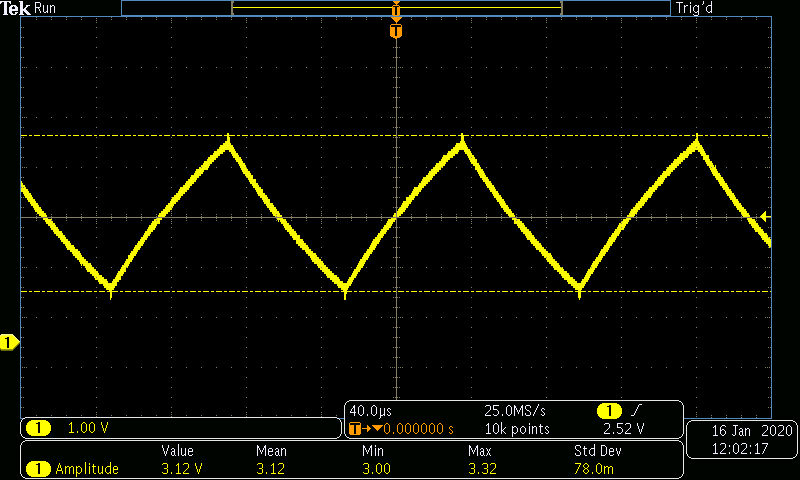
\includegraphics[width=0.8\textwidth]{graphics/Resolver_Dreieck.png}
	\caption{Dreiecksignal nach dem ersten Opamp.} 
	\label{fig:Hardware_Resolver_Interface_2}
\end{figure}
\newpage
Abbildung \ref{fig:Hardware_Resolver_Interface_3} zeigt das angenäherte Sinussignal, welches auf die Erregerspule geführt wird. Das Signal hat mit 3.6V$_{PP}$, im Gegensatz zur Simulation mit 4.8V$_{PP}$, eine zu kleine Amplitude. Es ist zu erkennen, dass das Signal oben und unten abgeschnitten ist. Die Gründe dafür konnten nicht herausgefunden werden, können bei Bedarf im Projekt 6 herausgefunden werden. Da die Rede war, für das Projekt 6 einen Motor mit ABN-Encoder zu verwenden, könnte auf diesen Schritt verzichtet werden. Ein Einfluss könnten die unterschiedlichen Widerstände machen, welche den Spannungsteiler am positiven Anschluss des Opamps bilden.

\begin{figure}[h!]
	\centering
	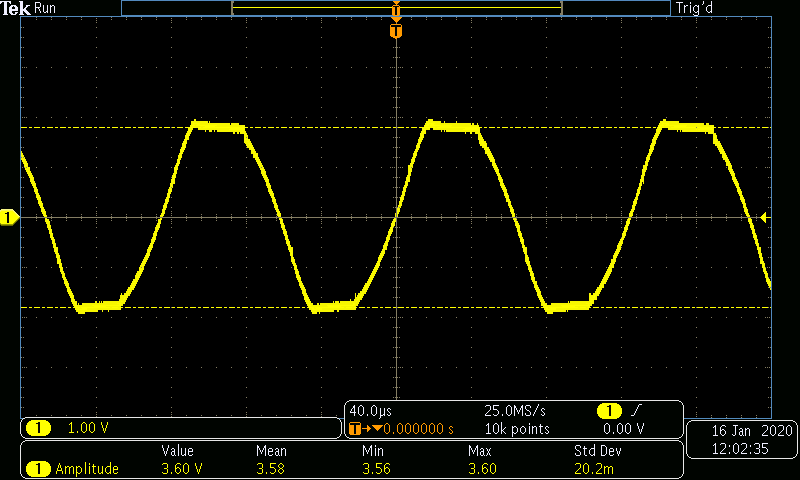
\includegraphics[width=0.8\textwidth]{graphics/Resolver_Sin_Aus.png}
	\caption{Angenähertes Sinussignal nach dem zweiten Opamp.} 
	\label{fig:Hardware_Resolver_Interface_3}
\end{figure}

Abbildung \ref{fig:Hardware_Resolver_Interface_4} zeigt das einkommende Signal der Sinusspule am Resolver. Die Signalform hat sich durch die Induktivitäten im Resolver verbessert. Es hat eine Amplitude von 1.18V$_{PP}$, was im Gegensatz zur simulierten Amplitude von 2.4V$_{PP}$. Somit ist die Übertragungsamplitude nicht 2:1, sondern 3.6:1.12. Möglicherweise liegt dies am nicht sauberen Ausgangssignal und einer kleinen Verschiebung der Messspule zur Erregerspule.

\begin{figure}[h!]
	\centering
	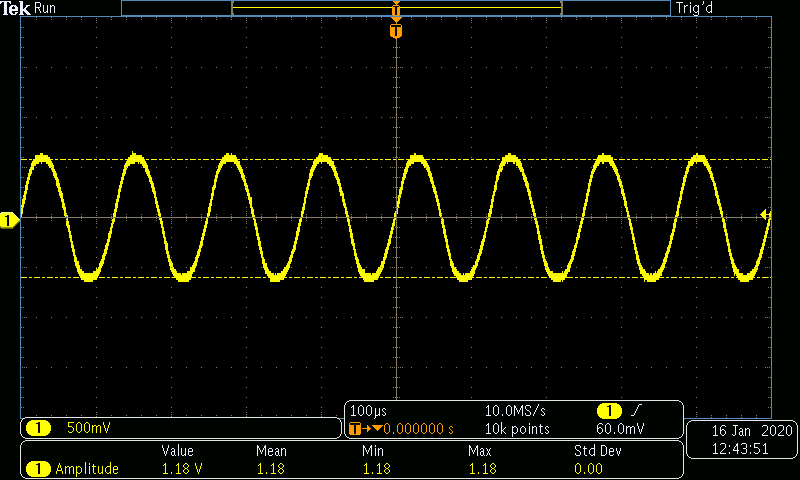
\includegraphics[width=0.8\textwidth]{graphics/Resolver_Sin_Ein_1.png}
	\caption{Rückkehrendes Signal aus Resolver.} 
	\label{fig:Hardware_Resolver_Interface_4}
\end{figure}
\newpage


Abbildung \ref{fig:Hardware_Resolver_Interface_5} zeigt das aufbereitete Signal für den Motorentreiber. Es hat eine Signalamplitude von 1.4V$_{PP}$ und einen Offset von 2.5V, was einen Spannungsbereich von 1.8V$_{PP}$ bis 3.2V$_{PP}$ ergibt. Dies liegt im Bereich des Treibers und kann theoretisch skaliert werden für die Verarbeitung der Signale. Die Schaltung ist somit ausreichend für den Resolver, kann jedoch noch verbessert werden.

\begin{figure}[h!]
	\centering
	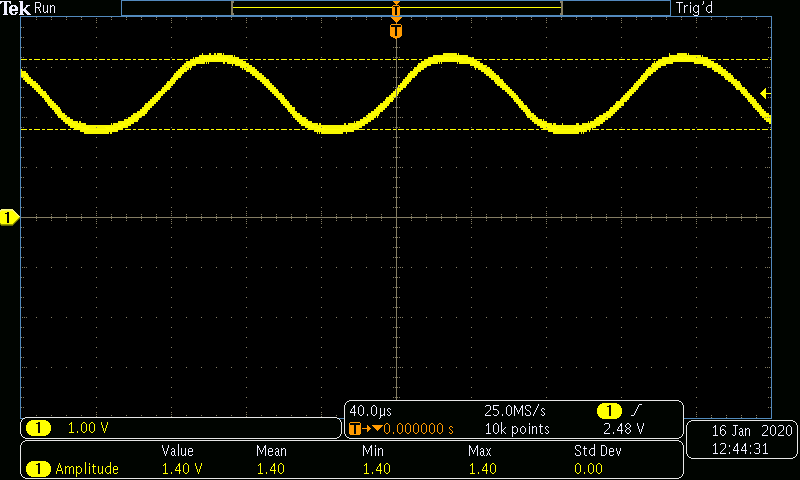
\includegraphics[width=0.8\textwidth]{graphics/Resolver_Sin_Verst_1.png}
%	\includegraphics[width=0.8\textwidth]{graphics/Messung_Resolver_Interface_4.png}
	\caption{Messung am Sinus-Eingang, aufbereitet für Mikrocontroller.} 
	\label{fig:Hardware_Resolver_Interface_5}
\end{figure}

Abbildung \ref{fig:Hardware_Resolver_Interface_6} zeigt das Signal der Cosinus Messpule. Es hat eingangsseitig eine Amplitude von 1.18V$_{PP}$ und ist auch hier tiefer als die errechneten 2.4V$_{PP}$.

\begin{figure}[h!]
	\centering
	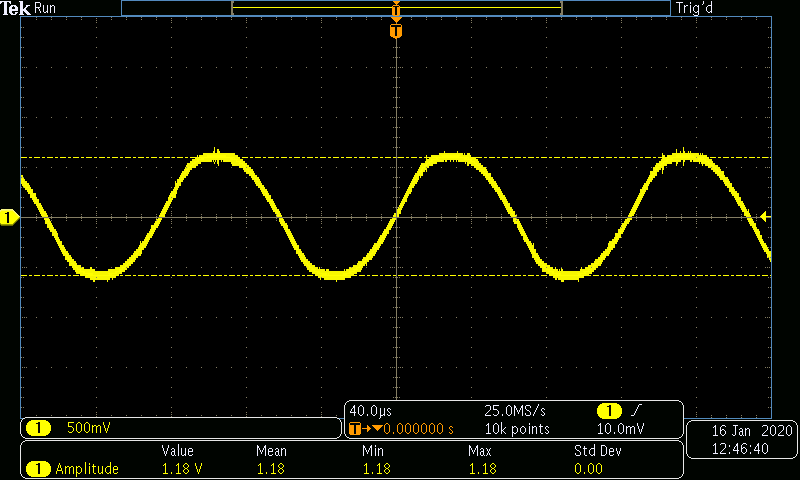
\includegraphics[width=0.8\textwidth]{graphics/Resolver_Sin_Ein_2.png}
	\caption{Messung am Cosinus-Eingang, aufbereitet für Mikrocontroller.} 
	\label{fig:Hardware_Resolver_Interface_6}
\end{figure}
\newpage
Abbildung \ref{fig:Hardware_Resolver_Interface_7} zeigt das aufbereitete Signal für den Motorentreiber. Es hat eine Signalamplitude von 1.4V$_{PP}$ und einen Offset von 2.5V, was einen Spannungsbereich von 1.8V$_{PP}$ bis 3.2V$_{PP}$ ergibt. Dies liegt im Bereich des Treibers und kann theoretisch skaliert werden für die Verarbeitung der Signale. Die Schaltung ist somit ausreichend für den Resolver, kann jedoch noch verbessert werden.

\begin{figure}[h!]
	\centering
	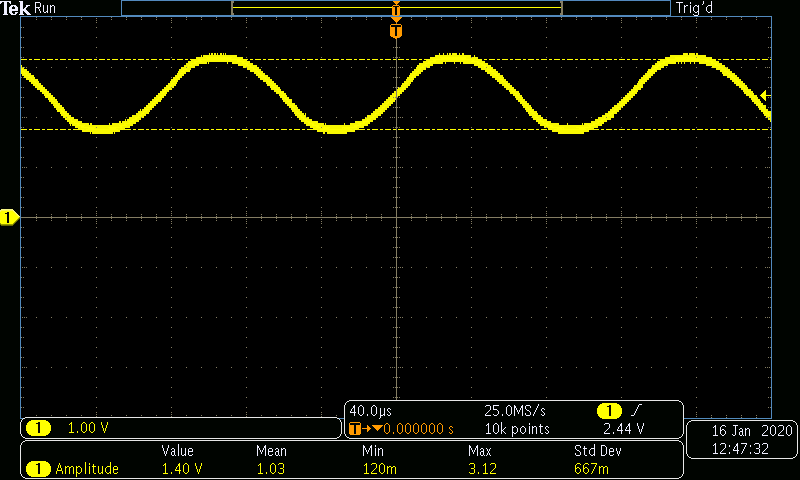
\includegraphics[width=0.8\textwidth]{graphics/Resolver_Sin_Verst_2.png}
%	\includegraphics[width=0.8\textwidth]{graphics/Messung_Resolver_Interface_4.png}
	\caption{Messung am Sinus-Eingang, aufbereitet für Mikrocontroller.} 
	\label{fig:Hardware_Resolver_Interface_7}
\end{figure}

Eine Implementierung des eingebauten Resolvers hat leider nicht geklappt, da die Eingangssignale nicht richtig verarbeitet werden konnten. So konnte der Motor nur im Torque- und Flux-Modus betrieben werden, was sehr zum Nachteil der Cocktailmaschine wäre. Darum wurde entschieden, mit einem ABN-Encoder zu arbeiten, um uns trotzdem mit dem Chip und seinen Möglichkeiten vertraut zu machen.

\subsubsection{TMC4671}\label{subsubse:Hardware_TMC4671}

Für die Ansteuerung wurde die Software \textit{TMCL-IDE 3.0} verwendet. Anfangs wurde der Motor in den Openloop versetzt. Danach wurden die Analogeingänge für die Strommessung skaliert, gefolgt von der Initialisierung des ABN-Encoders. Mit schrittweisem Erhöhen der PI-Parametern war es möglich, den Motor in verschiedenen Modi zu steuern. 

Der Torque-/Flux-Modus konnte mit Einstellen deren PI-Parametern gesteuert werden, bei Belastung drehte der Motor langsamer, das Drehmoment blieb das selbe.

Mit setzen der PI-Paramter des Velocity-Modus, war der Treiber in der Lage, bei ändernder Belastung den Rotor stets auf einer konstanten Drehzahl zu halten, indem er das Drehmoment erhöhte.

Bei Aktivierung des Position-Modus und setzen dessen PI-Parametern, konnte der Treiber den Rotor je nach Wert um einen gewissen Winkel drehen. 

Für den Bewegungsablauf ist es möglich, die Limits der Parameter zu setzen, um das Bewegungsverhalten zu kontrollieren. Im Falle der Cocktailmaschine dürfen die Bewegungen nicht zu abrupt sein, aber dürfen bei längeren Strecken auch zügiger vorangehen.

Aufgrund technischer Schwierigkeiten mit dem EVAL-Board , konnten leider keine Bilder der Software während des Betriebs gemacht werden.